\documentclass{article}

% PACKAGES
% General Formatting & Language
\usepackage[english]{babel}
\usepackage[letterpaper,top=2cm,bottom=2cm,left=3cm,right=3cm,marginparwidth=1.75cm]{geometry}
\usepackage{booktabs}
\usepackage{longtable}
\usepackage{multirow}
\usepackage{float}
\usepackage{placeins}


% Math & Symbols
\usepackage{amsmath}
\usepackage{amssymb}
\usepackage{amsthm}
\usepackage{bm}
\usepackage{bbold}

% Graphics & Colors
\usepackage{graphicx}
\usepackage{xcolor}
\usepackage[most]{tcolorbox}

% TikZ
\usepackage{tikz}
\usetikzlibrary{shapes, decorations.pathmorphing, shapes.geometric, calc, arrows.meta, positioning, backgrounds}
\usetikzlibrary{matrix,positioning,calc}


% Algorithms
\usepackage{algorithm}
\usepackage{algorithmic}

% Miscellaneous
\usepackage{enumitem}
\usepackage{url}
\usepackage{xr}
\externaldocument{main}
\usepackage[colorlinks=true, allcolors=blue]{hyperref}

% CUSTOM COMMANDS & THEOREMS
\newtheorem{lemma}{Lemma}
\newcommand{\hlm}[1]{{\color{blue}#1}}
\newcommand{\mbw}[1]{{\color{blue}#1}}
\newcommand{\ind}{\mathrel{\perp\!\!\!\!\perp}}

\title{Supplementary Material\\[0.4em]\large CICADAS: A Simulation-Based Framework for Randomized Trial Emulation in Critical-Care Seizure Treatment}


% \title{CICADAS \cicada: A Simulation-Based Tutorial for Causal Survival Analysis with Complex Time-Varying Confounding}

% \title{CICADAS: A Simulation-Based Tutorial for Causal Survival Analysis with Complex Time-Varying Confounding}


\author{
    Mitchell McCauley\textsuperscript{1*},
    Tara Westover\textsuperscript{2*}, 
    Patrick Wynn\textsuperscript{1*}, 
    Shadi Sartipi\textsuperscript{3*}, \\
    Niels Turley\textsuperscript{1},
    Zade Akras\textsuperscript{3},
    Pieter Colin\textsuperscript{4},
    Andrew Webb\textsuperscript{3}, 
    Aaron F. Struck\textsuperscript{5},
    Jennifer Kim\textsuperscript{6},\\ 
    David Cheng\textsuperscript{3}, % Manual line break for formatting
    Haoqi Sun\textsuperscript{1}, 
    Tim Houle\textsuperscript{3}, 
    Cynthia Rudin\textsuperscript{7}, 
    Alexander Volfovsky\textsuperscript{7}, Harsh Parikh\textsuperscript{6} \\
    Marta B. Fernandes\textsuperscript{3\dag}, % Manual line break for formatting
    Sahar Zafar\textsuperscript{3\dag},
    M.\ Brandon Westover\textsuperscript{1\dag}
}

\date{} % Suppress date

\begin{document}
\maketitle

\renewcommand{\thesection}{S\arabic{section}}
\renewcommand{\thetable}{S\arabic{table}}
\renewcommand{\thefigure}{S\arabic{figure}}
\setcounter{section}{0}\setcounter{table}{0}\setcounter{figure}{0}

\tableofcontents
\newpage

\section{Causal Identification: Derivations}
\subsection{Setup and assumptions}

\subsubsection{Structure of the observed data}
\label{sssec:structure-data}
Consider a longitudinal study observed at discrete times \(k = 0, 1, \ldots, K\). At each time \(k\), events occur in the following order:
\[
  X_k \;\;\longrightarrow\;\; A_k \;\;\longrightarrow\;\; Y_k \;\;\longrightarrow\;\; V_{k+1}.
\]

with a causal graph in which all past variables influence all future variables. The first two time steps of this graph are shown in Figure~\ref{fig:DAG-supp}.

\begin{figure}[H]
\centering
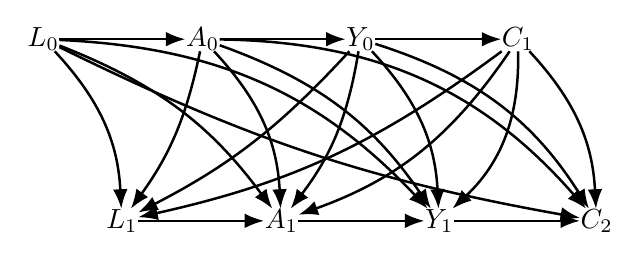
\begin{tikzpicture}[
  node distance = 1cm and 1.6cm,
  >=Latex, baseline,
  every node/.style={inner sep=0pt, anchor=center},
  main/.style={line width=0.9pt, draw=black},
  uniform/.style={line width=0.9pt, draw=black}
]
  % ----- time-0 nodes -----
  \node (L0) {$L_{0}$};
  \node[right=of L0] (A0) {$A_{0}$};
  \node[right=of A0] (Y0) {$Y_{0}$};
  \node[right=of Y0] (C1) {$C_{1}$};
  % ----- time-1 nodes (shifted right) -----
  \node[below=2cm of L0, xshift=1cm] (L1) {$L_{1}$};
  \node[right=of L1] (A1) {$A_{1}$};
  \node[right=of A1] (Y1) {$Y_{1}$};
  \node[right=of Y1] (C2) {$C_{2}$};
  % ----- within-time arrows (order inside each interval) -----
  \draw[->,uniform] (L0) -- (A0);
  \draw[->,uniform] (A0) -- (Y0);
  \draw[->,uniform] (Y0) -- (C1);
  \draw[->,uniform] (L1) -- (A1);
  \draw[->,uniform] (A1) -- (Y1);
  \draw[->,uniform] (Y1) -- (C2);
  % ----- cross-time "same-variable" persistence -----
  \draw[->,uniform,bend left=20] (L0) to (L1);
  \draw[->,uniform,bend left=20] (A0) to (A1);
  \draw[->,uniform,bend left=20] (Y0) to (Y1);
  \draw[->,uniform,bend left=20] (C1) to (C2);
  % ----- cross-time: all past → all future (now uniform black) -----
  % from L0
  \draw[->,uniform,bend left=16] (L0) to (A1);
  \draw[->,uniform,bend left=22] (L0) to (Y1);
  \draw[->,uniform,bend right=8] (L0) to (C2);
  % from A0
  \draw[->,uniform,bend left=12] (A0) to (L1);
  \draw[->,uniform,bend left=18] (A0) to (Y1);
  \draw[->,uniform,bend left=24] (A0) to (C2);
  % from Y0
  \draw[->,uniform,bend left=10] (Y0) to (L1);
  \draw[->,uniform,bend left=14] (Y0) to (A1);
  \draw[->,uniform,bend left=20] (Y0) to (C2);
  % from C1
  \draw[->,uniform,bend left=12] (C1) to (L1);
  \draw[->,uniform,bend left=18] (C1) to (A1);
  \draw[->,uniform,bend left=24] (C1) to (Y1);
\end{tikzpicture}
\caption{Causal graph for the data.}
\label{fig:DAG-supp}
\end{figure}

Specifically:

\begin{itemize}
    \item \(X_k\) is a vector of covariates measured at time \(k\).
    \item \(A_k\) is the treatment assigned at time \(k\).
    \item \(Y_k\) is an indicator that the primary outcome has occurred by time \(k\). Thus, \(Y_k = 1\) means the event (of interest) was observed by or at time \(k\), and \(Y_k = 0\) otherwise.
    \item \(V_{k+1}\) is an indicator denoting whether the individual remains \emph{uncensored} immediately \emph{after} time \(k\). 
    Typically, \(V_{k+1} = 0\) means “still uncensored by time \(k+1\)”, while \(V_{k+1} = 1\) means the subject is censored at or before \(k+1\).
\end{itemize}

We let \(\bar{X}_k = (X_0, X_1, \ldots, X_k)\), \(\bar{A}_k = (A_0, A_1, \ldots, A_k)\), \(\bar{Y}_k=(Y_0, Y_1,\ldots, Y_k)\), and \(\bar{V}_k=(V_0, V_1, \ldots,V_k)\).  By convention, we set \(V_0 = 0\) for all individuals (nobody is censored before baseline).  

\paragraph{Note on indexing.}
There are \(K+1\) total \emph{treatment times}: \(k=0,\dots,K\).  No new exposure is assigned \emph{after} time \(K\).  The final outcome is assessed at time \(K+1\). Hence, we write the treatment sequence as \(\bar{A} = (A_0,\dots,A_K)\) rather than extending to \(A_{K+1}\).  
\paragraph{Note on censoring.}
We consider two variants:
\begin{enumerate}
  \item Total effect: \(V_{k+1} = \bigl(C_{k+1}, D_{k+1}\bigr)\), where \(C_{k+1}\) indicates administrative censoring or loss to follow-up and \(D_{k+1}\) indicates a competing event (e.g.\ death).
  \item Direct effect: \(V_{k+1} = C_{k+1}\) alone, treating any competing event the same way as any other form of censoring (or truncation by death).
\end{enumerate}
The algebraic derivation is the same, but the interpretation of the causal contrast (direct or total effect) and the form of the equation representing \(V\) differ depending on which components are included in \(V\).  

\subsubsection{Definitions of causal effects}
\label{sssec:causal-effects}

Let \(g = (g_0, \ldots, g_K)\) denote a deterministic intervention, regime, or treatment strategy (static or dynamic) on \(A_k\) that may depend on the past measured covariate and treatment history, and that also sets to zero or eliminates the censoring process in \(V\).  For notational simplicity, we denote 
\[
   a^g_k \;=\; g_k\bigl(\bar{x}_k, \bar{a}^g_{k-1}\bigr),
\]
meaning that at each time \(k\), the intervention function \(g_k\) assigns the exposure \(A_k\) based on the treatment and covariate values in the past.  An individual’s full exposure sequence under \(g\) is \(\bar{a}^g = (a^g_0,a^g_1,\dots,a^g_K)\).  Likewise, under the hypothetical elimination of censoring (and possibly competing events), the counterfactual outcome is denoted
\[
  Y^g \equiv Y_{K+1}^{\bar{a}^g, \,\bar{v} = 0}.
\]
Here, “\(\bar{v} = 0\)” indicates an intervention that sets \(V_{k+1}=0\) for all \(k\), i.e.\ no individual is censored (which, in Case 1, also means individual ever has a competing event). 

Our goal in typical applications is to compare the risk or mean of \(Y_{K+1}\) under two or more possible intervention rules.  For instance, we might define a dynamic rule “treat whenever \(X_k\) is above some threshold”.  
% In one derivation below, we \(V_{k+1} = (C_{k+1}, D_{k+1})\), so that the intervention \(\bar{v}=0\) \emph{eliminates} both censoring and competing events (death).  In another, we let \(V_{k+1} = C_{k+1}\) alone, so that we only eliminate censoring, while letting competing events occur as in the natural course.

\subsubsection{Identifying assumptions and the g-formula}
\label{sssec:identifying}

Throughout, we assume three conditions that allow identification via the g-formula (for each \(k=0,\dots,K\)):

\begin{tcolorbox}[title= Identification Conditions, breakable, enhanced jigsaw]

\begin{enumerate}
    \item \textbf{Exchangeability.}  
      \[
         (Y_{k+1}^g,\ldots,Y_{K+1}^g)
         \;\;\amalg\;\; \bigl(A_k, \,V_{k+1}\bigr)
         \;\bigm|\; \bar{X}_k = \bar{x}_k, \,\bar{A}_{k-1} = \bar{a}^g_{k-1},\,V_k=Y_k=0.
      \]
      In words, once we adjust for the past \((X,A)\) among individuals who remain in the study \(\bigl(V_k =0\bigr)\) and have not yet experienced \(Y=1\), the counterfactual outcome is independent of how the next exposure \(A_k\) or censoring/competing-event indicator \(V_{k+1}\) is realized.

    \item \textbf{Positivity.}
      The statement below is written in the discrete-case form (point mass on the intervention
      value \(a_k^g\)) for notational simplicity. When \(A_k\) is continuous, it should be read
      as the continuous-neighborhood overlap condition given in \S 2.2 of the main text, which
      reduces to the discrete form when \(A_k\) is discrete.
      \begin{align*}
              & f_{\bar{X}_k,\,\bar{A}_{k-1},\,V_k,\,Y_k}\bigl(\bar{x}_k,\,\bar{a}_k,\,0,\,0\bigr)\neq 0  \implies  \\
              & P\Bigl(A_k = a^g_k,\; V_{k+1}=0 \;\bigm|\; \bar{X}_k=\bar{x}_k,\; \bar{A}_{k-1}=\bar{a}^g_{k-1},\; V_k = Y_k = 0\Bigr) > 0.
      \end{align*}

      In words: at any time \(k\) with a positive-density observed history, the mechanism
      assigning treatment and censoring must have positive probability of producing the value
      demanded by the intervention (or any value in its neighborhood) while remaining alive
      and uncensored.

    \item \textbf{Consistency.}   
      \[\bar{A}_K = \bar{a}^g_K, \quad \bar{V}_{K+1}=0 \implies   \bar{X}_K =\bar{X}_K^g, \quad Y_{K+1} \;=\;Y_{K+1}^g.\] 
      That is, if the intervention \(\bar{A}^g\) and censoring elimination \(\bar{v}=0\) match the observed data, then the observed outcome agrees with its counterfactual counterpart.
\end{enumerate}
\end{tcolorbox}

Under these assumptions, the counterfactual risk or mean of \(Y_{K+1}\) 
under any intervention \(\bar{A}^{g,\bar{v}=0}\) is identified by the g-formula.



%  --------------------------------
% Get rid of everything after this?
%  --------------------------------

\begin{align*}
  \Pr\bigl(Y_{K+1}^{g,\bar{c}=0} = 1\bigr)
  &=\;
  \sum_{\bar{x}_K}\;\sum_{k=0}^{K}
  \Pr\Bigl(Y_{k+1}=1 \,\Big|\,\bar{X}_k=\bar{x}_k,\;\bar{Y}_k=0,\;\bar{C}_{k+1}=0,\;\bar{A}_k=\bar{a}_k
  \Bigr) \\
    &\quad\times\;
    \prod_{j=0}^{k}
      \Pr\Bigl(Y_j=0 \,\Big|\,
        \bar{X}_j=\bar{x}_j,\;\bar{Y}_{j-1}=0,\;\bar{C}_j=0,\;\bar{A}_j=\bar{a}_j
      \Bigr) \\
      &\quad\times\;
      f\Bigl(x_j \,\Big|\,
        \bar{x}_{j-1},\;\bar{Y}_{j-1}=0,\;\bar{C}_j=0,\;\bar{A}_{j-1}=\bar{a}_{j-1}
        \Bigr)
  \\[6pt]
\end{align*}

We consider two cases, corresponding to different choices of the censoring vector \(C_{k+1}\):
\\
\begin{itemize}
  \item \emph{Total effect}: If we set \(C_{k+1} = \bigl(C_{k+1}, D_{k+1}\bigr)\), where \(C_{k+1}\) indicates loss to follow-up and \(D_{k+1}\) indicates a competing event, then the g-formula gives the \emph{total effect} of the intervention \(g\) on the outcome \(Y\): the effect that would be observed if the intervention were implemented and all censoring and competing events were eliminated. In this case, the g-formula is given by Corollary 1. 
          

  \item \emph{Direct effect}: If we set \(V_{k+1} = C_{k+1}\), 
        this indicates that we with estimate the effect after eliminate censoring due to loss to follow up 
        but not due to the competing event. 
        In that setting, if the subject experiences \(D_k=1\) before \(Y\), they are removed from the risk set.  
        In this setting, we group the competing event with the time-varying covariates, 
        \(X_{k} = (L_k,D_k)\). Then the g-formula is given by Corollary 2.
        

\end{itemize}


All derivations in this appendix follow from these core assumptions and definitions, using the standard arguments for the g-formula and for its IPW representation (see, e.g., Robins 1986; Hernán and Robins 2020). 
\begin{tcolorbox}[title=Theorem 1: General g-formula for a time-varying treatment with elimination of censoring, breakable, enhanced jigsaw]
    \label{thm:timevarying_gformula}
    Consider a deterministic (static or dynamic) intervention $g$ that sets $\bar{A}_k = \bar{a}_k^g$ for all $k = 0,\ldots,K$. 
    Assume that for all individuals the identifying assumptions hold (exchangeability, positivity, consistency).
    Then the counterfactual risk under \(\bar{a}^g\) and elimination of censoring is given by
  
    \begin{align*}
      \Pr\bigl(Y_{K+1}^{g} = 1\bigr)
      &=\;
      \sum_{\bar{x}_K} \sum_{k=0}^K 
          \Pr\Bigl(Y_{k+1} = 1 \,\Big|\,\bar{X}_k = \bar{x}_k,\;\bar{A}_k=\bar{a}^g_k,\; \bar{Y}_k=0,\;\bar{V}_{k+1}=0 \Bigr) \\[6pt]
      &\quad\quad \times\;
      \prod_{j=0}^{k} \Pr\Bigl(Y_j=0 \,\Big|\, \bar{X}_{j-1} = \bar{x}_{j-1},\;\bar{A}_{j-1} = \bar{a}^g_{j-1},\;\bar{Y}_{j-1} = \bar{V}_j = 0 \Bigr) \\[6pt]
      &\quad\quad\quad \times\;
        f\Bigl(x_j \,\Big|\,\bar{x}_{j-1},\;\bar{A}_{j-1} = \bar{a}^g_{j-1},\; \bar{Y}_{j} =\bar{V}_j = 0 \Bigr)
    \end{align*}
        
        
    \begin{align*}
      \Pr\bigl(Y_{K+1}^{g} = 0\bigr)
      &=\;
      \sum_{\bar{x}_K} \Pr\Bigl(Y_{K+1} = 0 \,\Big|\,\bar{X}_K = \bar{x}_K,\;\bar{A}_K=\bar{a}^g_k,\; \bar{Y}_K=0,\;\bar{V}_{K+1}=0 \Bigr) \\[6pt]
      &\quad \times
      \prod_{j=0}^{K} \Pr\Bigl(Y_j=0 \,\Big|\, \bar{X}_{j-1} = \bar{x}_{j-1},\;\bar{A}_{j-1} = \bar{a}^g_{j-1},\; \bar{Y}_{j-1} = 0,\;\bar{V}_j = 0 \Bigr) \\[6pt]
      &\quad\quad \times\;
        f\Bigl(x_j \,\Big|\,\bar{x}_{j-1},\;\bar{A}_{j-1} = \bar{a}^g_{j-1},\; \bar{Y}_{j} = 0,\;\bar{V}_j = 0 \Bigr)
    \end{align*}
        
        

    \end{tcolorbox}

\paragraph{Proof.}
Let $\bar{A}_{t-1} = \bar{a}^g_{t-1}$, $t \leq k$. 
If $f(\bar{L}_t,\bar{A}_{t-1},V_t = 0,Y_t = 0) \neq 0$ 
then define 
$b^g(k,t) = \Pr[Y^g_{k+1} = 0|\bar{L}_t,\bar{A}_{t-1},V_t = Y_t = 0]$. 
Note that 
$b^g(k,-1) = \Pr[Y^g_{k+1} = 0]$ 
as $\bar{X}_{-1} = \bar{A}_{-2} = \bar{V}_{-1} = \bar{Y}_{-1} = 0$ by definition. Then:
\begin{flalign*}
    b^g(k,t) &\stackrel{a}{=} \Pr[Y^g_{t+1} = \cdots = Y^g_{k+1} = 0|\bar{X}_t,\bar{A}_{t-1},Y_t = V_t = 0] \\
    &\stackrel{b}{=} \Pr[Y^g_{t+1} = \cdots = Y^g_{k+1} = 0|\bar{X}_t,\hlm{\bar{A}_{t}},Y_t = \hlm{V_{t+1}}= 0] \\
    &\stackrel{c}{=} \Pr[\hlm{Y^g_{t+1} = 0}|\bar{X}_t,\bar{A}_{t},Y_t = V_{t+1} = 0] \times \Pr[Y^g_{t+2} = \cdots = Y^g_{k+1} = 0|\bar{X}_t,\bar{A}_{t}, \hlm{Y_{t+1}} =V_{t+1} =  0]  \\
    &\stackrel{d}{=} \Pr[\hlm{Y_{t+1} = 0}|\bar{X}_t,\bar{A}_{t},Y_t = V_{t+1} = 0] \times \Pr[Y^g_{t+2} = \cdots = Y^g_{k+1} = 0|\bar{X}_t,\bar{A}_{t}, Y_{t+1} =V_{t+1} =  0]  \\
    &\stackrel{e}{=} \hlm{\sum_{x_{t+1}}}\Pr[Y_{t+1} = 0|\bar{X}_t,\bar{A}_{t},Y_t = V_{t+1} = 0] \times \Pr[\hlm{X_{t+1}}, Y^g_{t+2} = \cdots = Y^g_{k+1} = 0|\bar{X}_t,\bar{A}_{t}, Y_{t+1} =V_{t+1} =  0]  \\
    &\stackrel{f}{=} \sum_{x_{t+1}} \Pr[Y_{t+1} = 0|\bar{X}_t,\bar{A}_{t},Y_t = V_{t+1} = 0] \\
    & \quad\quad  \times \Pr[Y^g_{t+2} = \cdots = Y^g_{k+1} = 0|\hlm{\bar{X}_{t+1}},\bar{A}_{t}, Y_{t+1} =V_{t+1} =  0]  \\
    &\quad\quad \times f(\hlm{x_{t+1}}|\bar{x}_t, \bar{a}^g_t,V_{t+1} = Y_{t+1} = 0) \\
    &\stackrel{g}{=} \sum_{x_{t+1}}
    \Pr[Y_{t+1} = 0|\bar{X}_t,\bar{A}_{t},Y_t = V_{t+1} = 0]\\
    & \quad\quad  \times \Pr[Y^g_{t+2} = \cdots = Y^g_{k+1} = 0|\bar{X}_{t+1},\hlm{\bar{A}_{t+1}}, Y_{t+1} =\hlm{V_{t+2}} =  0]  \\
    &\quad\quad \times f(x_{t+1}|\bar{a}^g_t,\bar{x}_t,V_{t+1} = Y_{t+1} = 0) \\
    &\stackrel{h}{=} \sum_{x_{t+1}}\hdots \sum_{x_{k}}
    \Pr[ Y^g_{k+1} = 0|\bar{X}_{k},\bar{A}_{k}, Y_{k} =V_{k+1} =  0] \\
    & \quad\quad \times \prod_{j=t+1}^k \Pr[Y_{t+1} = 0|\bar{X}_t,\bar{A}_{t},Y_t = V_{t+1} = 0]  \\
    &\quad\quad\quad\quad\quad \times f(x_{t+1}|\bar{a}^g_t,\bar{x}_t,V_{t+1} = Y_{t+1} = 0), \\
\end{flalign*}
where (a) is because $Y^g_{k+1}=0$ implies $Y^g_{t+1} = \cdots = Y^g_{k} = 0$, (b) is by positivity and exchangeability, (c) is by rules of probability, and consistency, (d) is by the law of total probability, (e) is by the rules of probability, and (f) follows by iterating the preceding steps. Plugging $t=-1$ into $b^g(k,t)$ gives the desired expression for $\Pr[Y^{g}_{K+1}=0]$. For the other expression, we note that $\Pr[Y^g_{K+1}=1] = \sum_{k=0}^K \Pr[Y^g_{k+1}=1]\Pr[\bar{Y}^g_{k}=0]$, and then follow steps similar to those above. \(\blacksquare\) 
\begin{tcolorbox}[title=Corollary 1: Direct effect under elimination of death and censoring]
    \label{cor:direct-effect-time-varying}
    
  Let $V_k = (C_k,D_k)$, $X_k = L_k$, 
  assume the order of events at each time step is $L_k, A_k, Y_k, D_{k+1}, C_{k+1}$,
  and consider a hypothetical intervention $g$ 
  eliminates both censoring and death. 
  For each individual, assume the three identifying 
  conditions hold. Then the direct effect of the intervention $g$ on the survival outcome at time $K+1$ is given by:

  
  \begin{align*}
      P\Bigl(Y_{K+1}^g &= 1\Bigr) \;=\;
      P\Bigl(Y^{\bar{a}^g,\bar{c}=\bar{d}=0} = 1\Bigr) \\
      & = \sum_{\bar{l}_K} \; \sum_{k=0}^{K}\;
      \Pr\Bigl(Y_{k+1} = 1 \,\Bigm|\,
              \bar{L}_k=\bar{l}_k,\;\bar{A}_k=\bar{a}^g_k,\;
              \bar{Y}_k = \bar{C}_{k+1}=\bar{D}_{k+1}=0\Bigr)
      \\
      & \qquad \times \;
      \prod_{j=0}^{k}
      \Bigl\{\,
        \Pr\Bigl(Y_j=0 \,\Bigm|\,
                \bar{L}_{j-1}=\bar{l}_{j-1},\;\bar{A}_{j-1}=\bar{a}^g_{j-1},\;
                \bar{Y}_{j-1} = 
                \bar{C}_j=\bar{D}_j=0\Bigr)
      \\
      &\qquad\qquad\qquad \times\;
        f\Bigl(l_j \,\Bigm|\,
                  \bar{l}_{j-1},\;\bar{A}_{j-1}=\bar{a}^g_{j-1},\;
                  \bar{C}_j=\bar{D}_j=\bar{Y}_j=0\Bigr)
      \Bigr\},
  \end{align*}  
    where for \(j=0\),  
    \(
    f\Bigl(l_0 \,\Bigm|\,
       \bar{C}_0 = \bar{D}_0 = \bar{Y}_0=0,\; \bar{A}_{-1}=0\Bigr)
      \;\equiv\;
    f(l_0),
    \)
    the marginal distribution of baseline covariates.
    
    \end{tcolorbox}
    
    \noindent
    \textbf{Proof.}
    This result follows immediately from Theorem~1.  Specifically, we take
    \(\,V_{k+1} = (C_{k+1}, D_{k+1})\)
    and
    \(X_k = L_k\).
    \(\blacksquare\)
    
\begin{tcolorbox}[title=Corollary 2: Total effect: g-formula under elimination of censoring but not death] 

    Let $V_k = C_k$, and $X_k = (L_k,D_{k+1})$, assume the order
    of events at each time step is $L_k, A_k, Y_k, D_{k+1},  C_{k+1}$,
    and consider a hypothetical intervention $g$ 
    eliminates censoring but not death. 
    For each individual, assume the three identifying 
    conditions hold. Then the total effect of the intervention $g$ on the survival outcome at time $K+1$ is given by:
  
    \begin{align*}
        P\Bigl(Y_{K+1}^g &= 1\Bigr) \;=\;
        P\Bigl(Y^{\bar{a}^g,\bar{c}=0} = 1\Bigr) \\
        & = \sum_{\bar{l}_K} \; \sum_{k=0}^{K}\;
        \Pr\Bigl(Y_{k+1} = 1 \,\Bigm|\,
                \bar{L}_k=\bar{l}_k,\;\bar{A}_k=\bar{a}^g_k,\;
                \bar{Y}_k=\bar{C}_{k+1}=\bar{D}_{k+1}=0\Bigr)
        \\
        & \qquad \times \;
        \prod_{j=0}^{k}
        \Bigl\{\,
          \Pr\Bigl(Y_j=0 \,\Bigm|\,
                  \bar{L}_{j-1}=\bar{l}_{j-1},\;\bar{A}_{j-1}=\bar{a}^g_{j-1},\;
                  \bar{Y}_{j-1} = \bar{C}_j=\bar{D}_j = 0\Bigr)
        \\
        &\qquad\qquad \times\;
          \Pr\Bigl(D_{j+1}=0 \,\Bigm|\,
                \bar{L}_{j}=\bar{l}_{j},\;\bar{A}_j=\bar{a}^g_j,\;
                \bar{Y}_j = \bar{C}_{j+1}=\bar{D}_j=0 \Bigr)        \\
        &\qquad\qquad \times\;
          f\Bigl(l_j \,\Bigm|\,
                    \bar{l}_{j-1},\;\bar{a}^g_{j-1},\;
                    \bar{Y}_j=\bar{C}_j=\bar{D}_j=0\Bigr)
        \Bigr\},
    \end{align*}  


\end{tcolorbox}



\textbf{Proof}. Setting $\bar{X}_k = (\bar{L}_k,\,\bar{D}_{k+1})$ in Theorem 1, we get: 

\begin{align*}
        \Pr\bigl(Y_{K+1}^{g} = 1\bigr)
        &\stackrel{a}{=}\;
        \sum_{\bar{x}_K, \bar{d}_{K+1}} \sum_{k=0}^K 
            \Pr\Bigl(Y_{k+1} = 1 \,\Big|\,\hlm{\bar{L}_k = \bar{l}_k,\;\bar{D}_{k+1}=\bar{d}_{k+1}},\;\bar{A}_k=\bar{a}^g_k,\; \bar{Y}_k=0,\;\bar{V}_{k+1}=0 \Bigr) \\[6pt]
        &\quad\quad \times\;
        \prod_{j=0}^{k} \Pr\Bigl(Y_j=0 \,\Big|\, \hlm{\bar{L}_{j-1} = \bar{l}_{j-1},\;\bar{D}_{k}=\bar{d}_k},\;\bar{A}_{j-1} = \bar{a}^g_{j-1},\;\bar{Y}_{j-1} = \bar{V}_j = 0 \Bigr) \\[6pt]
        &\quad\quad\quad \times\;
          f\Bigl(\hlm{l_j,d_{j+1}}) \,\Big|\,\hlm{\bar{l}_{j-1},\;d_{j}},\; \bar{A}_{j-1} = \bar{a}^g_{j-1},\; \bar{Y}_{j} =\bar{V}_j = 0 \Bigr)\\
          &\stackrel{b}{=}\;
          \sum_{\bar{x}_K, \bar{d}_{K+1}} \sum_{k=0}^K 
              \Pr\Bigl(Y_{k+1} = 1 \,\Big|\,\bar{L}_k = \bar{l}_k,\;\bar{D}_{k+1}=\bar{d}_{k+1},\;\bar{A}_k=\bar{a}^g_k,\; \bar{Y}_k=0,\;\bar{V}_{k+1}=0 \Bigr) \\[6pt]
          &\quad\quad \times\;
          \prod_{j=0}^{k} \Pr\Bigl(Y_j=0 \,\Big|\, \bar{L}_{j-1} = \bar{l}_{j-1},\;\bar{D}_{k}=\bar{d}_k,\;\bar{A}_{j-1} = \bar{a}^g_{j-1},\;\bar{Y}_{j-1} = \bar{V}_j = 0 \Bigr) \\[6pt]
          &\quad\quad\quad \times\;
            \hlm{f\Bigl(l_j \Big|\,\bar{l}_{j-1},\;d_{j},\; \bar{A}_{j-1} = \bar{a}^g_{j-1},\; \bar{Y}_{j} =\bar{V}_j = 0 \Bigr)}\\
        &\quad\quad\quad \times\;
        \hlm{\Pr(D_{j+1}=d_{j+1} \,\Big|\,\bar{l}_{j},\;\bar{D}_j = \bar{d}_{j},\; \bar{A}_{j-1} = \bar{a}^g_{j-1},\; \bar{Y}_{j} =\bar{V}_j = 0 \Bigr)}\\
        &\stackrel{c}{=}\;
          \sum_{\bar{x}_K, \bar{d}_{K+1}} \sum_{k=0}^K 
              \Pr\Bigl(Y_{k+1} = 1 \,\Big|\,\bar{L}_k = \bar{l}_k,\;\bar{D}_{k+1}=\bar{d}_{k+1},\;\bar{A}_k=\bar{a}^g_k,\; \bar{Y}_k=0,\;\bar{V}_{k+1}=0 \Bigr) \\[6pt]
          &\quad\quad \times\;
          \prod_{j=0}^{k} \Pr\Bigl(Y_j=0 \,\Big|\, \bar{L}_{j-1} = \bar{l}_{j-1},\;\bar{D}_{k}=\bar{d}_k,\;\bar{A}_{j-1} = \bar{a}^g_{j-1},\;\bar{Y}_{j-1} = \bar{V}_j = 0 \Bigr) \\[6pt]
          &\quad\quad\quad \times\;
            f\Bigl(l_j \Big|\,\bar{l}_{j-1},\;d_{j},\; \bar{A}_{j-1} = \bar{a}^g_{j-1},\; \bar{Y}_{j} =\bar{V}_j = 0 \Bigr)\\
        &\quad\quad\quad \times\;
        \Pr\Bigl(D_{j+1}=d_{j+1} \,\Big|\,\bar{l}_{j},\;\bar{D}_j = \bar{d}_{j},\; \hlm{\bar{A}_{j} = \bar{a}^g_{j}},\; \bar{Y}_{j} =\bar{V}_j = 0 \Bigr)\\
        &\stackrel{d}{=}\;
        \hlm{\sum_{\bar{x}_K}} \sum_{k=0}^K 
              \Pr\Bigl(Y_{k+1} = 1 \,\Big|\,\bar{L}_k = \bar{l}_k,\;\hlm{\bar{D}_{k+1}=0},\;\bar{A}_k=\bar{a}^g_k,\; \bar{Y}_k=0,\;\bar{V}_{k+1}=0 \Bigr) \\[6pt]
          &\quad\quad \times\;
          \prod_{j=0}^{k} \Pr\Bigl(Y_j=0 \,\Big|\, \bar{L}_{j-1} = \bar{l}_{j-1},\;\hlm{\bar{D}_{k}=0},\;\bar{A}_{j-1} = \bar{a}^g_{j-1},\;\bar{Y}_{j-1} = \bar{V}_j = 0 \Bigr) \\[6pt]
          &\quad\quad\quad \times\;
            f\Bigl(l_j \Big|\,\bar{l}_{j-1},\;\hlm{\bar{D}_{j}=0},\; \bar{A}_{j-1} = \bar{a}^g_{j-1},\; \bar{Y}_{j} =\bar{V}_j = 0 \Bigr)\\
        &\quad\quad\quad \times\;
        \Pr\Bigl(\hlm{D_{j+1}=0} \,\Big|\,\bar{l}_{j},\;\hlm{\bar{D}_j = 0},\; \bar{A}_{j} = \bar{a}^g_{j},\; \bar{Y}_{j} =\bar{V}_j = 0 \Bigr),
\end{align*}
where (a) is by substitution of $V_k = C_k$ and $X_k = (L_k,D_{k+1})$ into Theorem 1; (b) is by rules of probability; (c) is because $\bar{A}_j = \bar{a}_j^g$ is a deterministic function of $\bar{l}_j$ and $\bar{a}^g_{j-1}$, that is $a_j^g=g_j(\bar{l}_j,\bar{a}^g_{j-1})$; and (d) is because $Y_{k+1}=1$ can only occur if $D_j=0$ for all $j=0,\ldots,k$, thus all sequences of $d_j$ drop out of the sum except the all-zeros sequence. \(\blacksquare\) 
\begin{tcolorbox}[title=Corollary 3: g-formula for competing event]

    Let $g$ be a deterministic intervention that eliminates censoring and imposes treatment $a^g_k = g_k(\bar{l}_k,\bar{a}^g_{k-1})$, and assume the following identifying assumptions hold:
    \begin{enumerate}
        \item \textbf{Exchangeability.}  
          \[
             (D_{k+1}^g,\ldots,D_{K+1}^g)
             \;\;\amalg\;\; \bigl(A_k, \,C_{k+1}\bigr)
             \;\bigm|\; \bar{L}_k = \bar{l}_k, \,\bar{A}_{k-1} = \bar{a}^g_{k-1},\,C_k=Y_k=0.
          \]
    
        \item \textbf{Positivity.}
          (As in Appendix Theorem~1, the statement below is written in the discrete-case form;
          for continuous \(A_k\) it is interpreted as the continuous-neighborhood overlap
          condition of \S 2.2 of the main text.)
          \begin{align*}
                  & f_{\bar{L}_k,\,\bar{A}_{k-1},\,C_k,\,D_k}\bigl(\bar{l}_k,\,\bar{a}_k,\,0,\,0\bigr)\neq 0  \implies  \\
                  & P\Bigl(A_k = a^g_k,\; C_{k+1}=0 \;\bigm|\; \bar{L}_k=\bar{l}_k,\; \bar{A}_{k-1}=\bar{a}^g_{k-1},\; C_k = Y_k = 0\Bigr) > 0
          \end{align*}
    
    
        \item \textbf{Consistency.}   
          \[\bar{A}_K = \bar{a}^g_K, \quad \bar{C}_{K+1}=0 \implies   \bar{L}_K =\bar{L}_K^g, \quad Y_{K+1} \;=\;Y_{K+1}^g,\] 
        where we are taking $\bar{Y}_k$ to be an implicit component of $\bar{L}_k$. 
    \end{enumerate}

    Then the counterfactual risk of death by $K+1$ under $\bar{a}^g_k$ and elimination of censoring is given by
  
    \begin{align*}
      \Pr\bigl(D_{K+1}^{g} = 1\bigr)
      &=\;
      \sum_{\bar{l}_K} \sum_{k=0}^K 
          \Pr\Bigl(D_{k+1} = 1 \,\Big|\,\bar{L}_k = \bar{l}_k,\;\bar{A}_k=\bar{a}^g_k,\; \bar{D}_k=0,\;\bar{C}_{k+1}=0 \Bigr) \\[6pt]
      &\quad\quad \times\;
      \prod_{j=0}^{k} \Pr\Bigl(D_j=0 \,\Big|\, \bar{L}_{j-1} = \bar{l}_{j-1},\;\bar{A}_{j-1} = \bar{a}^g_{j-1},\;\bar{D}_{j-1} = \bar{C}_j = 0 \Bigr) \\[6pt]
      &\quad\quad\quad \times\;
        f\Bigl(l_j \,\Big|\,\bar{l}_{j-1},\;\bar{A}_{j-1} = \bar{a}^g_{j-1},\; \bar{D}_{j} =\bar{C}_j = 0 \Bigr)
    \end{align*}
    
    Similarly, the counterfactual probability of survival up to $K+1$ under $\bar{a}^g_k$ and elimination of censoring is given by
    \begin{align*}
      \Pr\bigl(D_{K+1}^{g} = 0\bigr)
      &=\;
      \sum_{\bar{l}_K} \Pr\Bigl(D_{K+1} = 0 \,\Big|\,\bar{L}_K = \bar{l}_K,\;\bar{A}_K=\bar{a}^g_k,\; \bar{D}_K=0,\;\bar{C}_{K+1}=0 \Bigr) \\[6pt]
      &\quad \times
      \prod_{j=0}^{K} \Pr\Bigl(D_j=0 \,\Big|\, \bar{L}_{j-1} = \bar{l}_{j-1},\;\bar{A}_{j-1} = \bar{a}^g_{j-1},\; \bar{D}_{j-1} = 0,\;\bar{C}_j = 0 \Bigr) \\[6pt]
      &\quad\quad \times\;
        f\Bigl(l_j \,\Big|\,\bar{l}_{j-1},\;\bar{A}_{j-1} = \bar{a}^g_{j-1},\; \bar{D}_{j} = 0,\;\bar{C}_j = 0 \Bigr)
    \end{align*}

\end{tcolorbox}

\textbf{Proof:} The result follows from Theorem 1 by replacing $\bar{Y}_{k+1}$, $\bar{V}_{k+1}$, $\bar{X}_k$ and the corresponding counterfactuals from Theorem 1 with $\bar{D}_{k+1}$, $\bar{C}_{k+1}$, $\bar{L}_k$ and their corresponding counterfactuals, respectively $\blacksquare$
\subsection{Derivation of the Monte Carlo Implementation of the Parametric G-Formula}
\label{app:gformula_derivation}

Here provide a brief derivation showing why forward simulation from
the disease-evolution model generates sample paths from the post-intervention
covariate distribution $f^g(\bar{L}_K)$, and why Monte Carlo averaging over such
trajectories yields a valid numerical implementation of the parametric g-formula.

\subsubsection{Factorization of the Post-Intervention Covariate Distribution}

Consider a deterministic dynamic treatment policy
$g = (g_0,\ldots,g_K)$, where at each time $t$ the treatment is assigned as
$A_t = g_t(\bar{L}_t,\bar{A}_{t-1})$.
Under the assumptions of consistency, sequential ignorability, and positivity,
the joint distribution of the covariate history under policy $g$ and no censoring,
$f^g(\bar{l}_K)$, is identified by the g-formula.

By repeated application of the chain rule and conditioning on survival and lack
of censoring up to each time point, this distribution admits the factorization
\begin{align}
f^g(\bar{l}_K)
&=
f(l_0)
\prod_{t=0}^{K-1}
f\!\left(
l_{t+1}
\,\middle|\,
\bar{l}_t,\,
\bar{a}^g_t,\,
\bar{C}_t = \bar{Y}_t = 0
\right),
\label{eq:fg_factorization}
\end{align}
where $\bar{a}^g_t = (a^g_0,\ldots,a^g_t)$ is the treatment history induced by policy
$g$. Sequential ignorability ensures that each conditional density in
\eqref{eq:fg_factorization} coincides with the corresponding conditional density
estimable from the observed data-generating process.

\subsubsection{G-Formula for Discrete-Time Survival}

For a discrete-time survival outcome, the probability of surviving through time
$K+1$ under policy $g$ can be written as
\begin{align}
P(Y^g_{K+1} = 0)
&=
\sum_{\bar{l}_K}
\left[
\prod_{t=0}^{K}
P\!\left(
Y_{t+1} = 0,\,
C_{t+1} = 0
\,\middle|\,
\bar{L}_t = \bar{l}_t,\,
\bar{A}_t = \bar{a}^g_t,\,
\bar{C}_t = \bar{Y}_t = 0
\right)
\right]
f^g(\bar{l}_K).
\label{eq:gformula_survival}
\end{align}

Substituting the factorization of $f^g(\bar{l}_K)$ from
\eqref{eq:fg_factorization} into \eqref{eq:gformula_survival} yields an expression
for $P(Y^g_{K+1} = 0)$ as an expectation with respect to the post-intervention
covariate distribution.

\subsubsection{Monte Carlo Approximation}

Equation \eqref{eq:gformula_survival} involves a summation over all possible
covariate trajectories $\bar{l}_K$, which is computationally infeasible in
all but trivial settings. However, because $f^g(\bar{l}_K)$ is fully specified
by the product of conditional transition densities in
\eqref{eq:fg_factorization}, we can generate independent draws
$\bar{l}^{(1)}_K,\ldots,\bar{l}^{(M)}_K \sim f^g(\bar{L}_K)$
by recursively simulating
\[
L_{t+1}^{(m)} \sim
f\!\left(
L_{t+1}
\,\middle|\,
\bar{L}^{(m)}_t,\,
\bar{A}^{g}_t,\,
\bar{C}_t = \bar{Y}_t = 0
\right),
\qquad
t = 0,\ldots,K-1,
\]
with $A_t = g_t(\bar{L}^{(m)}_t,\bar{A}^{(m)}_{t-1})$.

The g-formula integral can then be approximated by the Monte Carlo estimator
\begin{align}
P(Y^g_{K+1} = 0)
&\approx
\frac{1}{M}
\sum_{m=1}^{M}
\prod_{t=0}^{K}
P\!\left(
Y_{t+1} = 0,\,
C_{t+1} = 0
\,\middle|\,
\bar{L}_t = \bar{l}^{(m)}_t,\,
\bar{A}_t = \bar{a}^g_t,\,
\bar{C}_t = \bar{Y}_t = 0
\right),
\end{align}
which converges almost surely to the true g-formula estimand as
$M \to \infty$ by the law of large numbers.

Thus, forward simulation from the disease-evolution model under policy $g$,
followed by averaging of the corresponding survival probabilities, constitutes
a valid numerical implementation of the parametric g-formula.


\subsection{Relation to Alternative G-Formula Estimators}
\paragraph{Relation to alternative g-formula estimators.}
The g-formula estimand in \eqref{eq:gformula_survival1} can also be targeted by other
estimators, including inverse probability of treatment and censoring weighting (IPTW),
iterated conditional expectations, and parametric plug-in estimators
\cite{hernan2020causal}. In the present setting, however, IPTW can be unstable for
continuous, state-dependent dosing policies over long horizons due to extreme weights
and near-positivity violations, while iterated expectation and direct plug-in approaches
require evaluating high-dimensional nested conditional expectations. By contrast,
forward Monte Carlo simulation from the disease-evolution model provides a numerically
stable and conceptually direct implementation that aligns with the mechanistic PK/PD and
disease-dynamics models used throughout CICADAS.

In the following sections, we present specific disease evolution and outcome models
that capture the ICU seizure treatment scenario, methods for estimating their
parameters, and experimental results using these models to estimate and optimize
treatment effects.



\subsection{IPW Formulas}\label{sec:appendix-ipw}
\begin{tcolorbox}[title=Lemma 1: General IPW formula]

Define
\[h_k^{v=0}(\bar{a}^g_k) = \frac{E[Y_{k+1}(1 - Y_k)W_k^V|\bar{A}_k = \bar{a}^g_k]}{E[(1 - Y_k)W_k^V|\bar{A}_k = \bar{a}^g_k]},\]

\noindent and
\begin{align*}
W_k^V = \prod_{j=0}^k \frac{I(V_{j+1} = 0)}{Pr[V_{j+1} = 0|\bar{X}_j, \bar{A}_k = \bar{a}^g_j, \bar{Y}_j = \Bar{V}_j = 0]},
\end{align*}

\noindent Then for $k = 0, \ldots, K$,
\begin{align*}
&h_k^{v=0}(\bar{a}^g_k) \prod_{j=0}^{k-1} [1 - h_j^{v=0}(\bar{a}^g_j)] \\ 
&= E[Y_{k+1}(1 - Y_k)W_k^V|\bar{A}_k = \bar{a}^g_k] \\
& \quad \times \prod_{j=1}^k \frac{E[(1 - Y_{j-1})W_{j-1}^V|\bar{A}_k = \bar{a}^g_{j-1}] - E[Y_j(1 - Y_{j-1})W_{j-1}^V|\bar{A}_k = \bar{a}^g_{j-1}]}{E[(1 - Y_j)W_j^V|\bar{A}_k = \bar{a}^g_j]}
\end{align*}
\end{tcolorbox}

\textbf{Proof.} For brevity, we will write = $\bar{a}^g_k$ in place of $\bar{A}_k = \bar{a}^g_k$. For  $0 \leq t < k - 1$, we have
\begin{align}
h_k^{v=0}(\bar{a}^g_k) \prod_{j=t}^{k-1} [1 - h_j^{v=0}(\bar{a}^g_j)] &= \frac{E[Y_{k+1}(1 - Y_k)W_k^V|\bar{a}^g_k]}{E[(1 - Y_k)W_k^V|\bar{a}^g_k]} \nonumber\\
&\quad \times \left\{1 - \frac{E[Y_k(1 - Y_{k-1})W_{k-1}^V|\bar{a}^g_{k-1}]}{E[(1 - Y_{k-1})W_{k-1}^V|\bar{a}^g_{k-1}]}\right\} \nonumber\\
&\quad \times \ldots \times \left\{1 - \frac{E[Y_{t+1}(1 - Y_t)W_t^V|\bar{a}^g_t]}{E[(1 - Y_t)W_t^V|\bar{a}^g_t]}\right\} \nonumber\\
&= \frac{E[Y_{k+1}(1 - Y_k)W_k^V|\bar{a}^g_k]}{E[(1 - Y_k)W_k^V|\bar{a}^g_k]} \nonumber\\
&\quad \times \left\{\frac{E[(1 - Y_{k-1})W_{k-1}^V|\bar{a}^g_{k-1}] - E[Y_k(1 - Y_{k-1})W_{k-1}^V|\bar{a}^g_{k-1}]}{E[(1 - Y_{k-1})W_{k-1}^V|\bar{a}^g_{k-1}]}\right\} \nonumber\\
&\quad \times \ldots \times \left\{\frac{E[(1 - Y_t)W_t^V|\bar{a}^g_t] - E[Y_{t+1}(1 - Y_t)W_t^V|\bar{a}^g_t]}{E[(1 - Y_t)W_t^V|\bar{a}^g_t]}\right\} \nonumber\\
&= \frac{E[Y_{k+1}(1 - Y_k)W_k^V|\bar{a}^g_k] \times \{E[(1 - Y_{k-1})W_{k-1}^V|\bar{a}^g_{k-1}] - E[Y_k(1 - Y_{k-1})W_{k-1}^V|\bar{a}^g_{k-1}]\}}{E[(1 - Y_k)W_k^V|\bar{a}^g_k]} \nonumber\\
&\quad \times \frac{\{E[(1 - Y_{k-2})W_{k-2}^V|\bar{a}^g_{k-2}] - E[Y_{k-1}(1 - Y_{k-2})W_{k-2}^V|\bar{a}^g_{k-2}]\}}{E[(1 - Y_{k-1})W_{k-1}^V|\bar{a}^g_{k-1}]} \nonumber\\
&\quad \times \ldots \times \frac{\{E[(1 - Y_t)W_t^V|\bar{a}^g_t] - E[Y_{t+1}(1 - Y_t)W_t^V|t]\}}{E[(1 - Y_{t+1})W_{t+1}^V|\bar{a}^g_{t+1}]} \nonumber\\
&\quad \times \frac{1}{E[(1 - Y_t)W_t^V|\bar{a}^g_t]} \nonumber\\
&= E[Y_{k+1}(1 - Y_k)W_k^V|\bar{a}^g_k] \nonumber\\
&\quad \times \left\{\prod_{j=t+1}^k \frac{E[(1 - Y_{j-1})W_{j-1}^V|\bar{a}^g_{j-1}] - E[Y_j(1 - Y_{j-1})W_{j-1}^V|\bar{a}^g_{j-1}]}{E[(1 - Y_j)W_j^V|\bar{a}^g_j]}\right\} \nonumber\\
&\quad \times \frac{1}{E[(1 - Y_t)W_t^V|\bar{a}^g_t]}
\end{align}

Our result follows by setting $t = 0$ and noting that $E[(1 - Y_0)W_0^V|\bar{a}^g_0] = 1$. \(\blacksquare\)
\begin{tcolorbox}[title=Theorem 1: IPW Lemma 2]
For \(k = 0, \ldots, K\) and \(W_k^V\) as in Lemma 1,
\[
E[(1 - Y_k)W_k^V\mid \bar{A}_k = \bar{a}^g_k] = E[(1 - Y_{k-1})W_{k-1}^V\mid \bar{A}_{k-1} = \bar{a}^g_{k-1}] - E[Y_k(1 - Y_{k-1})W_{k-1}^V\mid \bar{A}_{k-1} = \bar{a}^g_{k-1}].
\]
\end{tcolorbox}

\textbf{Proof:}

\begin{align*}
E&[(1 - Y_k)W_k^V\mid \bar{A}_k = \bar{a}^g_k] \\
&\stackrel{a}{=}  E\!\left[\,(1 - Y_k)W_{k-1}^V \, \frac{I(V_{k+1} = 0)}{P(V_{k+1} = 0\mid \bar{X}_k=\bar{x}_k, \bar{A}_k = \bar{a}^g_k, \bar{Y}_k = \bar{Y}_k=0)} \,\Bigg|\, \bar{A}_k = \bar{a}^g_k\right]\\
&\stackrel{b}{=}  E\!\left[(1 - Y_k)W_{k-1}^V\,\frac{E\![I(V_{k+1} = 0) \mid\, \bar{X}_k=\bar{x}_k, \bar{A}_k = \bar{a}^g_k, \bar{Y}_k = \bar{Y}_k=0]}{P(V_{k+1} = 0\mid \bar{X}_k=\bar{x}_k, \bar{A}_k = \bar{a}^g_k, \bar{Y}_k = \bar{Y}_k=0)} \,\Big|\bar{A}_k = \bar{a}^g_k\right] \\
&\stackrel{c}{=}  E\!\left[(1 - Y_k)W_{k-1}^V\,\frac{P(V_{k+1} = 0\mid \bar{X}_k=\bar{x}_k, \bar{A}_k = \bar{a}^g_k, \bar{Y}_k = \bar{Y}_k=0)}{P(V_{k+1} = 0\mid \bar{X}_k=\bar{x}_k, \bar{A}_k = \bar{a}^g_k, \bar{Y}_k = \bar{Y}_k=0)} \,\Big|\bar{A}_k = \bar{a}^g_k\right] \\
&=  E\!\left[(1 - Y_k)W_{k-1}^V\,\Big|\bar{A}_k = \bar{a}^g_k\right] \\
&\stackrel{d}=  E\!\left[(1 - Y_k)(1-Y_{k-1})W_{k-1}^V\,\Big|\bar{A}_k = \bar{a}^g_k\right] \\
 &=  E\!\left[(1 - Y_k)W_{k-1} - Y_k (1-Y_{k-1})W_{k-1}^V\,\Big|\bar{A}_k = \bar{a}^g_k\right] \\
&=  E\!\left[(1 - Y_k)W_{k-1}\Big|\bar{A}_k = \bar{a}^g_k\right] -E\!\left[ Y_k (1-Y_{k-1})W_{k-1}^V\,\Big|\bar{A}_k = \bar{a}^g_k\right], \\
\end{align*}
where (a) is by the definition of $W_{k}^V$, and (b) is by the law of iterated expectation: $E[A] = E[E[A|B]]$ To see why (c) is true, let $p = P(V_{k+1} = 0 \mid \bar{X}_k=\bar{x}_k, \bar{A}_k = \bar{a}^g_k, \bar{Y}_k = \bar{Y}_k=0)$. Conditioned on \((\bar{X}_k=\bar{x}_k, \bar{A}_k = \bar{a}^g_k, \bar{Y}_k = \bar{Y}_k=0)\), the indicator \(I(V_{k+1} = 0)\) is a Bernoulli random variable with parameter \(p\), it takes the value 1 with probability \(p\) and 0 with probability \(1-p\). Thus $ E\!\left[I(V_{k+1} = 0)\mid \bar{X}_k=\bar{x}_k, \bar{A}_k = \bar{a}^g_k, \bar{Y}_k = \bar{Y}_k=0\right] = p\cdot 1 + (1-p)\cdot0 = p$.
(d) is because $Y_k=0$ implies ($Y_k=0,Y_{k-1}=0$). \(\blacksquare\)

\begin{tcolorbox}[title=IPW Lemma 3]
For each \(k = 0, \ldots, K\),
\begin{align*}
E\Bigl[Y_{k+1}(1 - Y_k)W_k^V\mid \bar{A}_k = \bar{a}^g_k \Bigr] &= \sum_{\bar{x}_k} Pr\Bigl(Y_{k+1} = 1\mid \bar{X}_k = \bar{x}_k,\; \bar{A}_k = \bar{a}^g_k,\; \bar{Y}_k = \bar{V}_{k+1} = 0\;\Bigr) \nonumber\\
&\quad \times \prod_{j=0}^k Pr\Bigl(Y_j = 0\mid \bar{X}_{j-1} = \bar{x}_{j-1},\; \bar{A}_{j-1} = \bar{a}^g_{j-1},\; \bar{Y}_{j-1} = \bar{V}_j = 0\; \Bigr) \, \\
&\quad \quad \times f\Bigl(x_j\mid \bar{x}_{j-1}, \bar{A}_{j-1} = \bar{a}^g_{j-1}, \bar{Y}_j = \bar{V}_j = 0\; \Bigr),
\end{align*}
and
\begin{align*}
E\Bigl[(1 - Y_k)W_k^V\mid \bar{A}_k = \bar{a}^g_k\Bigr] &= \sum_{\bar{x}_{k-1}} Pr\Bigl(Y_k = 0\mid \bar{X}_{k-1} = \bar{x}_{k-1},\; \bar{A}_{k-1} = \bar{a}^g_{k-1},\; \bar{Y}_{k-1} = \bar{V}_k = 0\; \Bigr) \nonumber\\
&\quad \times \prod_{j=0}^{k-1} Pr\Bigl(Y_j = 0\mid \bar{X}_{j-1} = \bar{x}_{j-1},\; \bar{A}_{j-1} = \bar{a}^g_{j-1},\; \bar{Y}_{j-1} = \bar{V}_j = 0\; \Bigr) \\
& \quad \quad \times  f\Bigl(x_j\mid \bar{x}_{j-1}, \bar{A}_{j-1} = \bar{a}^g_{j-1},\; \bar{Y}_j = \bar{V}_j = 0\; \Bigr).
\end{align*}
\end{tcolorbox}

\textbf{Proof.} 
\begin{align*}
&E\Bigl[Y_{k+1}(1 - Y_k)W_k^V\mid \bar{A}_k=\bar{a}_k\Bigr] \\
&\stackrel{a}{=}\sum_{\bar{y}_{k+1}}\sum_{\bar{x}_k}\sum_{\bar{v}_{k+1}} y_{k+1}(1-y_k)
\left[\prod_{j=0}^k \frac{I(v_{j+1}=0)}{Pr(V_{j+1}=0\mid x_j,\bar{A}_k = \bar{a}^g_k, \,V_j=Y_j=0)}\right] \, f\Bigl(\bar{y}_{k+1},\,\bar{x}_k,\,\bar{v}_{k+1}\mid \bar{A}_k=\bar{a}^g_k\Bigr) \\
&\stackrel{b}{=}\sum_{\bar{y}_{k+1}}\sum_{\bar{x}_k}\sum_{\bar{v}_{k+1}} y_{k+1}(1-y_k)
\left[\prod_{j=0}^k \frac{I(v_{j+1}=0)}{Pr(V_{j+1}=0\mid x_j,\bar{A}_k = \bar{a}^g_k, \,V_j=Y_j=0)}\right] \\
& \quad \quad \quad \times  \prod_{j=0}^k \, f\Bigl(x_j\mid \bar{x}_{j-1},\, \bar{a}^g_j, \bar{y}_j,\,\bar{v}_j \Bigr) \; f\Bigl(y_{j+1}\mid \bar{x}_j,\, \bar{a}^g_j, \bar{y}_j, \bar{v}_{j+1} \Bigr) \; f\Bigl(v_{j+1}\mid \bar{x}_j,\,\bar{a}^g_j, \bar{y}_j, \bar{v}_j \Bigr). \\
&\stackrel{c}{=}\sum_{\bar{x}_k} \Pr\Bigl[ Y_{k+1}=1|\bar{X}_k=\bar{x}_k, \bar{A}_k = \bar{a}^g_k, \bar{Y}_k=\bar{V}_{k+1}=0\Bigr] \\
&\times 
\left[\prod_{j=0}^k \frac{f\Bigl(y_{j+1}=0 \mid \bar{x}_j,\, \bar{a}^g_j, \bar{y}_j, \bar{v}_{j+1} \Bigr) \; Pr\Bigr(V_{j+1}=0\mid x_j,\bar{A}_k = \bar{a}^g_k, \,V_j=Y_j=0\Bigl)f\Bigl(x_j\mid \bar{x}_{j-1},\, \bar{a}^g_j, \bar{y}_j,\,\bar{v}_j \Bigr) }{Pr(V_{j+1}=0\mid x_j,\bar{A}_k = \bar{a}^g_k, \,V_j=Y_j=0)}\right]\\
&\stackrel{d}{=}\sum_{\bar{x}_k} Pr\Bigl(Y_{k+1} = 1\mid \bar{X}_k = \bar{x}_k,\; \bar{A}_k = \bar{a}^g_k,\; \bar{Y}_k = \bar{V}_{k+1} = 0\;\Bigr) \nonumber\\
&\quad \times \prod_{j=0}^k Pr\Bigl(Y_j = 0\mid \bar{X}_{j-1} = \bar{x}_{j-1},\; \bar{A}_{j-1} = \bar{a}^g_{j-1},\; \bar{Y}_{j-1} = \bar{V}_j = 0\; \Bigr) \, \\
&\quad \quad \times f\Bigl(x_j\mid \bar{x}_{j-1}, \bar{A}_{j-1} = \bar{a}^g_{j-1}, \bar{Y}_j = \bar{V}_j = 0\; \Bigr),
\end{align*}
where (a) is by definition of $W_k^V = \prod_{j=0}^k \frac{I(V_{j+1} = 0)}{Pr(V_{j+1} = 0\mid X_j,\,V_j = Y_j = 0,\,A = a)}$; (b) is by laws of probability; (c) is because the indicator functions \(I(v_{j+1}=0)\) ensure that only sequences with \(v_{j+1}=0\) for \(j=0,\ldots,k\) contribute, and the factor \(y_{k+1}(1-y_k)\) forces \(y_{k+1}=1\) and \(y_k=0\), so that the only nonzero contributions come from the sequences satisfying $\bar{Y}_k=0,y_{k+1}=1,\bar{V}_{k+1}=0$; (d) is by cancelation and changing notation to match the theorem statement.

The second equality follows from a similar derivation. 

\(\blacksquare\)
\begin{tcolorbox}[title= IPW Theorem 2: Equivalence of the IPW and g-formulae] 
$$\Pr \Bigl[Y^{a,\overline{v}=0}_{K+1}=1\Bigr] = \sum_{k=0}^K h_k^{v=0}(a)\prod_{j=0}^{k-1}[1-h_j^{v=0}(a)].$$
\end{tcolorbox}

\textbf{Proof.} For brevity, we write $\bar{a}^g_K$ in place of $\bar{A}_K = \bar{a}^g_K$. 
\begin{align*}
    &\sum_{k=0}^K h_k^{v=0}(a)\prod_{j=0}^{k-1}[1-h_j^{v=0}(a)]\\
    & \stackrel{a}{=} \sum_{k=0}^K E[Y_{k+1}(1-Y_k)W_k^V|\bar{a}^g_k]\prod_{j=1}^k\frac{E[(1-Y_{j-1})W_{j-1}^V|\bar{a}^g_k]-E[Y_j(1-Y_{j-1})W_{j-1}^V|\bar{a}^g_k]}{E[(1-Y_j)W_j^V|\bar{a}^g_k]} \\
    & \stackrel{b}{=} \sum_{k=0}^K E[Y_{k+1}(1-Y_k)W_k^V|\bar{a}^g_k]\prod_{j=1}^k\frac{E[(1-Y_j)W_j^V|\bar{a}^g_k]}{E[(1-Y_j)W_j^V|\bar{a}^g_k]} \\
    & = \sum_{k=0}^K E[Y_{k+1}(1-Y_k)W_k^V|\bar{a}^g_k]\\[6pt]
    &\stackrel{c}{=}\sum_{k=0}^K\sum_{\bar{x}_K} 
        \Pr\Bigl(Y_{k+1} = 1 \,\Big|\,\bar{X}_k = \bar{x}_k,\;\bar{A}_k=\bar{a}^g_k,\; \bar{Y}_k=0,\;\bar{V}_{k+1}=0 \Bigr) \\[6pt]
    &\quad\quad \times\;
    \prod_{j=0}^{k} \Pr\Bigl(Y_j=0 \,\Big|\, \bar{X}_{j-1} = \bar{x}_{j-1},\;\bar{A}_{j-1} = \bar{a}^g_{j-1},\;\bar{Y}_{j-1} = \bar{V}_j = 0 \Bigr) \\[6pt]
    &\quad\quad\quad \times\;
      f\Bigl(x_j \,\Big|\,\bar{x}_{j-1},\;\bar{A}_{j-1} = \bar{a}^g_{j-1},\; \bar{Y}_{j} =\bar{V}_j = 0 \Bigr) \\[8pt]
    &\stackrel{d}{=} \Pr\bigl(Y_{K+1}^{g} = 1\bigr)
\end{align*}
where (a) is by Lemma 1, (b) is by Lemma 2, (c) is by Lemma 3, and (d) is by Theorem 1. \(\blacksquare\)


\begin{tcolorbox}[title=Corollary 4: Equivalence of g-formula and IPW representation for direct effect]

\begin{align*}
\Pr& \Bigl[Y^{a,\bar{c} = \bar{d} = 0}_{K+1}=1\Bigr] 
= \sum_{l_K} \sum_{k=0}^K \Pr[Y_{k+1} = 1 \mid \bar{L}_k = \bar{l}_k, \bar{A}_k = \bar{a}^g_k, \bar{D}_{k+1}=\bar{Y}_k = \bar{C}_{k+1} = 0] \\
& \quad \quad \quad \quad\quad \quad \times \prod_{j=0}^{k} \left\{ \right.
\Pr[Y_j = 0 \mid \bar{L}_{j-1} = \bar{l}_{j-1}, \bar{A}_k = \bar{a}^g_k, \bar{Y}_{j-1} = \bar{D}_j = \bar{C}_j = 0] \\
& \quad \quad\quad \quad\quad \quad\quad \quad \times f(l_j \mid \bar{l}_{j-1}, \bar{A}_{j-1}=\bar{a}^g_{j-1}, \bar{D}_j = \bar{Y}_j = \bar{C}_j =0) 
\left. \right\} \\
& = \sum_{k=0}^K h_k(\bar{a}^g_k) \prod_{j=0}^{k-1} \left[1 - h_j(\bar{a}^g_j)\right],
\end{align*}

where
$$
h_k(a) = \frac{E[Y_{k+1}(1 - Y_k) W_k \mid \bar{A}_k = \bar{a}^g_k]}{E[(1 - Y_k) W_k \mid \bar{A}_k=\bar{a}^g_k]},
$$
and \(W_k = W^C_k \cdot W^D_k\), with

\begin{align*}
    W^C_k &= \prod_{j=0}^k \frac{I(C_{j+1} = 0)}{\Pr[C_{j+1} = 0 \mid \bar{L}_j = \bar{l}_j, \bar{A}_j = \bar{a}^g_j,  \bar{D}_j = \bar{Y}_j = \bar{C}_j =0]} \\
    W^D_k & = \prod_{j=0}^k \frac{I(D_{j+1} = 0)}{\Pr[D_{j+1} = 0 \mid \bar{L}_j = \bar{l}_j,\bar{A}_j = \bar{a}^g_j, \bar{D}_j = \bar{Y}_j =  \bar{C}_{j+1} =0]}.
\end{align*}
\end{tcolorbox}

\textbf{Proof.} The result follows from Theorem 2 by choosing \(\bar{V}_{K+1} = (\bar{C}_{K+1}, \bar{D}_{K+1})\) and \(\bar{X}_K = \bar{L}_K\), corresponding to a setting where both loss to follow-up and competing events are considered censoring events, and all time-varying covariates are included. 
\(\blacksquare\)
\begin{tcolorbox}[title=Corollary 5: Equivalence of g-formula and IPW representation for total effect]
\begin{align*}
\Pr& \Bigl[Y^{a}_{K+1}=1\Bigr] 
= \sum_{l_K} \sum_{k=0}^K \Pr[Y_{k+1} = 1 \mid \bar{L}_k = \bar{l}_k, \bar{A}_k = \bar{a}^g_k, \bar{Y}_k = \bar{C}_{k+1} = 0] \\
& \quad \quad \quad \quad\quad \quad \times \prod_{j=0}^{k} \left\{ \right.
\Pr[Y_j = 0 \mid \bar{L}_{j-1} = \bar{l}_{j-1}, \bar{A}_{j-1} = \bar{a}^g_{j-1}, \bar{C}_j = \bar{Y}_{j-1} = 0] \\
& \quad \quad\quad \quad\quad \quad\quad \quad \times \Pr[D_{j+1} = 0 \mid \bar{L}_j = \bar{l}_j, \bar{A}_j = \bar{a}^g_{j}, = \bar{Y}_j = \bar{C}_{j+1} = \bar{D}_j  = 0] \\
& \quad \quad\quad \quad\quad \quad\quad \quad \times f(l_j \mid \bar{l}_{j-1}, \bar{A}_{j-1} = \bar{a}^g_{j-1},  \bar{D}_j = \bar{Y}_j = \bar{C}_j = 0) 
\left. \right\} \\
& = \sum_{k=0}^K h'_k(\bar{a}^g_k) \prod_{j=0}^{k-1} \left[1 - h'_j(\bar{a}^g_j)\right],
\end{align*}
where
$$
h'_k(\bar{a}^g_k) = \frac{E[Y_{k+1}(1 - Y_k) W'_k \mid \bar{A}_k = \bar{a}^g_k]}{E[(1 - Y_k) W'_k \mid \bar{A}_k = \bar{a}^g_k]},
$$
and 
\begin{align*}
    W'_k &= \prod_{j=0}^k \frac{I(C_{j+1} = 0)}{\Pr[C_{j+1} = 0 \mid \bar{L}_j = \bar{l}_j, \bar{A}_j = \bar{a}^g_j, \bar{D}_j = \bar{Y}_j = \bar{C}_j = 0]}
\end{align*}
\end{tcolorbox}
\textbf{Proof.} The result follows from Theorem 2 by choosing \(\bar{V}_{K+1} = \bar{C}_{K+1}\) and \(\bar{X}_K = (\bar{L}_K, \bar{D}_K)\), corresponding to a setting where only loss to follow-up is treated as a censoring event and competing events are treated as outcomes. 
\(\blacksquare\)

\section{Full Model Specification}
The main text gives the defining equation for each component of the simulation model. This section
collects the complete parameterizations, including the censoring and treatment-assignment mechanisms
and the full table of model variables, symbols, and ground-truth values.
\subsection{Model Parameters}
Table~\ref{tab:model_vars} summarizes the variables and parameters used throughout the framework. 

\begin{longtable}{lp{10cm}}
\caption{Model Variables and Parameters} \label{tab:model_vars} \\
\toprule
\textbf{Symbol} & \textbf{Description} \\
\midrule
\endfirsthead
\multicolumn{2}{c}{\textit{(continued from previous page)}} \\
\toprule
\textbf{Symbol} & \textbf{Description} \\
\midrule
\endhead
\midrule
\multicolumn{2}{r}{\textit{(continued on next page)}} \\
\endfoot
\bottomrule
\endlastfoot
\multicolumn{2}{l}{\textbf{State Variables}} \\
$L_t$ & Observed disease intensity/burden \\
$L_{0,t}$ & Underlying disease intensity (without treatment) \\
$X_t$ & Drug concentration \\
$A_t$ & Treatment administration rate (physician's action) \\
$Y_t$ & Death indicator (absorbing state) \\
$C_t$ & Censoring indicator (e.g., treatment deviation) \\
\midrule
\multicolumn{2}{l}{\textbf{Patient Characteristics}} \\
Age & Patient age (years) \\
SOFA & Sequential Organ Failure Assessment score \\
\midrule
\multicolumn{2}{l}{\textbf{Disease Model Parameters}} \\
$h$ & Growth rate during early phase \\
$H$ & Peak disease intensity (carrying capacity) \\
$\alpha$ & Mean reversion strength of disease process \\
$\delta$ & Decay rate of disease after peak \\
$\sigma_{\text{early}}, \sigma_{\text{late}}$ & Volatility of disease process in early and late phases \\
$\tau$ & Volatility transition time constant \\
\midrule
\multicolumn{2}{l}{\textbf{PK/PD Parameters}} \\
$k_e$ & Drug elimination rate constant \\
$C_{50}$ & Drug concentration for 50\% effect (EC50) \\
$\gamma$ & Hill coefficient for drug effect steepness \\
$\beta^C_0, \beta^C_1, \beta^C_2$ & Coefficients defining $C_{50}$ based on baseline covariates \\
$\beta^\gamma_0, \beta^\gamma_1, \beta^\gamma_2$ & Coefficients defining $\gamma$ based on baseline covariates \\
\midrule
\multicolumn{2}{l}{\textbf{Control Parameters}} \\
$\theta$ & Disease control target threshold \\
$\kappa_i$ & Integral control gain for treatment adjustments \\
$A_{\max}$ & Maximum treatment administration rate (saturation) \\
\midrule
\multicolumn{2}{l}{\textbf{Mortality Model Parameters}} \\
$\alpha_0, \alpha_1$ & Baseline log-odds and time effect on mortality \\
$\alpha_2$ & Baseline effect of cumulative disease burden on mortality \\
$\alpha_3$ & Interaction effect of SOFA score on disease harm \\
$\alpha_4$ & Baseline effect of cumulative treatment on mortality \\
$\alpha_5$ & Interaction effect of age on treatment harm \\
\midrule
\multicolumn{2}{l}{\textbf{Censoring Model Parameters}} \\
$\beta_0$ & Baseline log-odds of censoring for treated patients \\
$\beta_1$ & Effect of cumulative treatment burden on censoring (treated patients) \\
$\beta_2$ & Effect of time on censoring risk (treated patients) \\
$\beta_3$ & Baseline log-odds of censoring for untreated patients \\
$\beta_4$ & Effect of cumulative disease burden on censoring (untreated patients) \\
$\beta_5$ & Effect of time on censoring risk (untreated patients) \\
$A_{\mathrm{norm}}$ & Normalization constant for cumulative treatment burden (e.g., 207 units) \\
$L_{\mathrm{norm}}$ & Normalization constant for cumulative disease burden (e.g., 24 units) \\
$T_{\max}$ & Time normalization constant (e.g., 170 hours)
\end{longtable}

\subsection{Censoring Model: Full Specification}

In simulating observational (non-RCT) data, as in the observational cohort of the main text, patients may be censored due to deviation from following the closed-loop control strategy. The censoring model specified in this section is used solely to generate realistic observational datasets for simulation and validation purposes. Its role is to induce informative dropout and treatment-dependent protocol deviation, reflecting common features of ICU data that bias naive survival analyses. When applying the parametric g-formula to an observed dataset under the identification assumptions in Section~\ref{sec:prelim} of the main text, an explicit censoring model is not required: outcome and disease-evolution models are estimated conditional on remaining alive and uncensored.

We model censoring using a discrete-time hazard function \( h^{(c)}_{i,t} \), defined as the probability that patient \( i \) becomes censored in interval \( (t, t+1) \) given that they are uncensored up to time \( t \):
\[
h^{(c)}_{i,t} = P\!\left(C_{i,t+1} = 1 \,\middle|\, C_{i,t} = 0, \,\bar{L}_{i,t}, \,\bar{A}_{i,t} \right).
\]

The logit of the censoring hazard depends on treatment status:

\begin{equation}
\text{logit}\,h^{(c)}_{i,t} =
\begin{cases}
\beta_0 + \beta_1 \left(\frac{\sum_{s=0}^{t} A_{i,s}}{A_{\mathrm{norm}}}\right) + \beta_2 \left(\frac{t}{T_{\max}}\right)^2, & \text{if } A_{i,t} >0 \ \text{(treated)}, \\[6pt]
\beta_3 + \beta_4 \left(\frac{\sum_{s=0}^{t} L_{i,s}}{L_{\mathrm{norm}}}\right) + \beta_5 \left(\frac{t}{T_{\max}}\right)^2, & \text{if } A_{i,t}=0 \ \text{(untreated)}.
\end{cases}
\end{equation}

This specification reflects a deliberately simplified censoring mechanism designed for simulation. 
Among untreated patients ($A_{i,t}=0$), censoring is driven by cumulative disease burden 
(e.g., patients becoming too ill to continue protocolized monitoring), whereas among treated patients 
($A_{i,t}>0$), censoring is driven primarily by cumulative treatment burden 
(e.g., toxicity, complications, or decisions to discontinue aggressive therapy) and time. 
Because treatment is preferentially initiated in sicker patients and modifies their disease trajectories, 
disease burden remains indirectly related to censoring in the treated group through its influence on treatment exposure. 
Our goal is not to reproduce a clinically exact censoring process, but to generate realistic, 
informative censoring that depends on time-varying prognostic factors in a way that challenges standard survival methods.

Here:
\begin{itemize}
    \item $\text{Rx}_i$ denotes the patient's baseline treatment assignment 
    (1 = treated, 0 = untreated) used for labeling or stratification; 
    in contrast, $A_{i,t}$ represents the time-varying treatment intensity 
    actually administered during the simulation.
    \item $\beta_0 = -5$ and $\beta_3 = -5$ are baseline log-odds of censoring 
    for treated and untreated patients, respectively.
    \item $\beta_1 = 2.0$ models treatment burden leading to discontinuation.
    \item $\beta_4 = 2.0$ models disease burden leading to dropout in untreated patients.
    \item $\beta_2 = 0.1$ and $\beta_5 = 1.5$ capture time-varying increases in censoring risk.
    \item $A_{\mathrm{norm}} = 207$ and $L_{\mathrm{norm}} = 24$ normalize cumulative exposures.
    \item $T_{\max} = 170$ hours scales the time variable.
\end{itemize}

This censoring mechanism is \emph{informative}, because it depends on cumulative treatment burden and cumulative disease burden, both of which are prognostic for mortality. This has important implications: Standard Kaplan--Meier estimates will be biased under this censoring process (Figure~\ref{fig:swimmer_survival_rct}B of the main text). By contrast, the parametric g-formula naturally accounts for informative censoring.

When simulating data in RCT mode, no censoring occurs (\( h^{(c)}_{i,t} = 0 \) for all \( i,t \)), preserving the integrity of the randomized comparison.


\subsection{Treatment Assignment Model: Full Specification}


To create realistic confounding by indication in the observational data, we model a biased treatment assignment mechanism that mimics clinical practice, where physicians preferentially treat patients with more severe disease. 
Although treatment $A_t$ is continuous in our simulation (representing a drug infusion rate dynamically adjusted under a closed-loop control policy), we first define a binary baseline assignment indicator 
($A_{i,0} > 0$ vs.\ $A_{i,0} = 0$) to determine which patients enter the treated versus untreated regime. 
Once assigned, treated patients receive a time-varying continuous treatment trajectory governed by the policy $g_t(\bar{L}_t, \bar{A}_{t-1})$ defined in Section~\ref{sec:pkpd_model}. 
This setup preserves the continuous nature of treatment while allowing us to simulate realistic confounding by indication at baseline.

The probability that patient $i$ receives treatment at baseline (i.e., $A_{i,0} > 0$) is determined by a logistic regression model incorporating features of the early disease trajectory and baseline covariates:
\begin{equation}
\begin{aligned}
\text{logit}\!\left[
P\!\left(A_{i,0} > 0 \,\middle|\, \bar{L}_{i,10}, \text{SOFA}_i, \text{Age}_i\right)
\right]
&= \beta_0 
+ \beta_1 \bar{L}_{i,\mathrm{early}} 
+ \beta_2 L_{i,\max} \\
&\quad
+ \beta_3 L_{i,\mathrm{growth}}
+ \beta_4 L_{i,\mathrm{slope}}
+ \beta_5 L_{i,\mathrm{accel}} \\
&\quad
+ \beta_6 \text{SOFA}_i 
+ \beta_7 \text{Age}_i 
+ \eta_i .
\end{aligned}
\end{equation}
where:
\begin{itemize}
    \item $\bar{L}_{i,\mathrm{early}}$ is the mean disease severity over the first 10 time points;
    \item $L_{i,\max}$ is the maximum disease severity in the early trajectory;
    \item $L_{i,\mathrm{growth}} = (L_{i,10} - L_{i,1}) / (L_{i,1} + 0.01)$ is the relative early growth rate;
    \item $L_{i,\mathrm{slope}}$ is the fitted linear slope of the early disease trajectory;
    \item $L_{i,\mathrm{accel}}$ is the change in slope (acceleration) across the early phase;
    \item $\eta_i \sim \mathcal{N}(0, 0.3^2)$ adds stochastic variation.
\end{itemize}

The coefficients were calibrated to create substantial but realistic confounding:
\begin{itemize}
    \item $\beta_0 = -0.5$ (baseline log-odds)
    \item $\beta_1 = 0.8$, $\beta_2 = 0.6$, $\beta_3 = 1.2$, $\beta_4 = 1.0$, $\beta_5 = 0.8$ (disease severity effects)
    \item $\beta_6 = 0.5$ (SOFA score effect)
    \item $\beta_7 = -0.3$ (age effect)
\end{itemize}

This mechanism produces substantial confounding by indication: treated patients have 1.9-fold higher mean disease severity and 1.2-fold faster disease progression rates in the first 20 hours compared to untreated patients, with treatment assignment probability of 71.7\% (substantial deviation from the 50\% expected under randomization). 
Age shows no significant association with treatment ($p = 0.66$), while baseline SOFA scores are mildly associated ($p = 0.04$). 
This confounding pattern ensures that naive analyses will show biased treatment effects, while properly adjusted causal inference methods can recover the true treatment effect.

Because treatment intensity $A_{i,t}$ remains continuous and dynamically updated throughout the simulated trajectory, the g-formula’s positivity assumption holds automatically by construction within the simulated range of feasible doses.

We emphasize that Sections~4.1--4.5 define a complete data-generating mechanism for simulation studies; only the disease-evolution and outcome models are required inputs for g-formula estimation in applied settings.



\section{Estimation Details}
This section gives the filter and smoother recursions, the expectation--maximization updates, the
alternative estimation strategies compared in the main text, the design diagnostics used to screen
patients for inclusion, uncertainty quantification, and implementation details.
\subsubsection*{Extended Kalman Filter (EKF) and Rauch--Tung--Striebel (RTS) smoother}
This subsection describes the estimation algorithm used to infer the latent untreated
disease trajectory $L_{0,i,t}$ from noisy, treatment-modulated observations $L_{i,t}$
within the state-space model defined above.
Because $L_{0,i,t}$ is not directly observed, likelihood evaluation requires integration
over latent state trajectories.
We therefore adopt a standard nonlinear state-space formulation in which the disease
dynamics define state evolution and the PK/PD model defines a nonlinear observation equation.
To perform tractable inference in this setting, we use an Extended Kalman Filter (EKF)
for forward filtering and a Rauch--Tung--Striebel (RTS) smoother for backward smoothing.
These are standard smoothing methods used here solely to support parameter estimation
(via EM) and are not, by themselves, causal-inference contributions of CICADAS.
Here, $Q_t$ denotes the process-noise covariance governing stochastic evolution of
$L_{0,i,t}$, and $R$ denotes the observation-noise variance (or covariance) in the
measurement model for $L_{i,t}$.

\paragraph{EKF prediction.}
With $\hat L_{0,i,t-1|t-1}$ and $P_{i,t-1|t-1}$,
the predicted state mean is obtained by discretizing the drift
$\mu(L,t)$ defined in Equation~\eqref{eq:disease_drift}:
\begin{align}
\hat L_{0,i,t|t-1}
&= \hat L_{0,i,t-1|t-1}
   + \mu\!\left(\hat L_{0,i,t-1|t-1},\, t\right)\,\Delta t, \\
P_{i,t|t-1}
&= F_t\, P_{i,t-1|t-1}\, F_t^\top + Q_t,
\end{align}
where
\[
F_t
= \left.\frac{\partial}{\partial L}
\Big[ L + \mu(L,t)\,\Delta t \Big]\right|_{L=\hat L_{0,i,t-1|t-1}}
\]
is the Jacobian of the discretized drift with respect to the latent state. Here $Q_t$ denotes the process noise covariance implied by the diffusion term
in Equation~\eqref{eq:disease_diffusion}, and $R$ denotes the observation noise
variance of the PK/PD measurement model.

\paragraph{EKF update.}
Linearizing $h(x,t)=x\,s_{x_t,i}$ around $\hat L_{0,i,t|t-1}$ gives the observation matrix
\[
H_{i,t} \;=\; \left.\frac{\partial}{\partial x} \big[x\, s_{x_t,i}\big]\right|_{x=\hat L_{0,i,t|t-1}} \;=\; s_{x_t,i}.
\]
Then
\begin{align}
K_{i,t} &= P_{i,t|t-1} H_{i,t}^\top \Big(H_{i,t} P_{i,t|t-1} H_{i,t}^\top + R\Big)^{-1}, \\
\hat L_{0,i,t|t} &= \hat L_{0,i,t|t-1} + K_{i,t}\Big[L_{i,t} - \hat L_{0,i,t|t-1}\, s_{x_t,i}\Big], \\
P_{i,t|t} &= \big(I - K_{i,t} H_{i,t}\big)\, P_{i,t|t-1}.
\end{align}

\paragraph{RTS smoother.}
Backward for $t=T-1,\dots,0$:
\begin{align}
J_{i,t} &= P_{i,t|t}\, F_{t+1}^\top \, P_{i,t+1|t}^{-1}, \\
\hat L_{0,i,t|T} &= \hat L_{0,i,t|t} + J_{i,t}\,\big(\hat L_{0,i,t+1|T} - \hat L_{0,i,t+1|t}\big), \\
P_{i,t|T} &= P_{i,t|t} + J_{i,t}\,\big(P_{i,t+1|T} - P_{i,t+1|t}\big)\, J_{i,t}^\top.
\end{align}

\subsubsection*{Expectation--Maximization (EM)}
We jointly estimate $\boldsymbol{\theta}$ and the latent trajectories $\{L_{0,i,t}\}$ with EM.

\paragraph{E-step.}
Run EKF/RTS for each patient to obtain $\{\hat L_{0,i,t|T},\, P_{i,t|T}\}_{t=0}^T$ and the lagged covariances needed for quadratic forms in the M-step.

\paragraph{M-step.}
\emph{Fixed effects:} with $C_i$ and $g_i$ defined by the mixed-effects maps in Section~\ref{sec:pkpd_model},
\begin{equation}
\hat{\boldsymbol{\beta}}^{(k+1)} 
= \arg\min_{\boldsymbol{\beta}}
\left\{
\sum_{i,t}\, \ell_{i,t}(\boldsymbol{\beta};\, \hat L_{0,i,t|T}) \;+\; 
\lambda \big\|\boldsymbol{\beta}-\boldsymbol{\beta}_{\text{prior}}\big\|_2^2
\right\},
\end{equation}
where $\ell_{i,t}$ is the negative log-likelihood contribution under the linear mixed-effects maps for $C_i$ and $g_i$.

\emph{Variance components (random effects):}
\begin{align}
\hat\sigma_C^{2\,(k+1)} &= \frac{1}{N} \sum_{i=1}^N \big(\hat C_i - \mathbf{x}_i^\top \hat{\boldsymbol{\beta}}_C\big)^2, \\
\hat\sigma_g^{2\,(k+1)} &= \frac{1}{N} \sum_{i=1}^N \big(\hat g_i - \mathbf{x}_i^\top \hat{\boldsymbol{\beta}}_g\big)^2,
\end{align}
with $\mathbf{x}_i=[1,\,\mathrm{age}_i^*,\,\mathrm{SOFA}_i^*]^\top$.

\emph{PK elimination $k_e$:} see ``Strategy~3 (Two-stage)" below. If $k_e$ is treated as unknown in the joint likelihood, we update it by a one-dimensional line search maximizing the expected complete-data log-likelihood; however, for numerical stability and identifiability we prefer the two-stage procedure.

Iterate until $\|\boldsymbol{\theta}^{(k+1)} - \boldsymbol{\theta}^{(k)}\|_2 < \varepsilon$ or a maximum number of iterations is reached.

\subsubsection*{Alternative estimation strategies}
We considered four different estimation strategies:

\paragraph{(1) Joint estimation.}
Maximize a penalized likelihood over all parameters,
\[
\mathcal{L}(\boldsymbol{\theta})
= 
\sum_{i,t} \log p\!\big(L_{i,t}\,\big|\, \boldsymbol{\theta}, \mathcal{H}_{i,t-1}\big)
\;-\;\lambda \|\boldsymbol{\theta}\|_2^2,
\]
noting that $k_e$ can be weakly identified in closed-loop--like data due to confounding with $C_{50,i},\gamma_i$.

\paragraph{(2) Oracle $k_e$.}
Fix $k_e$ (could be reasonable if \ $k_e$ is known from prior PK studies) and estimate only $\boldsymbol{\beta}$ (and $\sigma_C^2,\sigma_g^2$). This reduces the parameter space and improves conditioning.

\paragraph{(3) Two-stage (when $k_e$ is unknown).}
\emph{Stage 1 (standalone $k_e$):} identify dose-change events with $|A_{i,t}-A_{i,t-1}|>\delta_A$; for each such event, extract a window of length $T_w$ time points post-change and fit
\[
\hat{k}_{e,i}
= \arg\min_{k_e} 
\sum_{t \in \text{window}} \Big[L_{i,t} - \hat L_{i,t}\big(t \,|\, k_e\big)\Big]^2
\]
under a simplified transient model; then aggregate across patients via a weighted median
\[
\hat{k}_e = \mathrm{median}_w\{\hat{k}_{e,i}\}, \qquad w_i = 1/\mathrm{var}(\hat{k}_{e,i}).
\]
\emph{Stage 2 (fixed $k_e$):} treat $\hat k_e$ as known and estimate $\boldsymbol{\beta},\sigma_C^2,\sigma_g^2$ via the EM steps above.

\paragraph{(4) Two-stage with bias correction.}
If $\hat k_e$ shows empirical bias, apply a calibrated multiplicative correction
\[
\hat k_e^{\text{corr}} \;=\; \alpha_{\mathrm{corr}} \cdot \hat k_e^{\text{raw}}, 
\quad \alpha_{\mathrm{corr}} = 1.41,
\]
optionally blending with prior information:
\[
\hat k_e^{\text{final}} \;=\; (1-w)\,\hat k_e^{\text{corr}} \;+\; w\, k_e^{\text{prior}}, \quad w \in [0,1].
\]

\subsubsection*{Design diagnostics and inclusion criteria}
We compute the design diagnostics in Section~\ref{sec:design_diagnostics} to verify estimability: sufficient time with $x_t/C_{50}$ in $[0.25,4]$, a 3--5x within-patient concentration span, and nonzero dose-change frequency. Only trajectories meeting minimal excitation are used for PK/PD estimation; others are held out for the survival analysis. 

\subsubsection*{Uncertainty quantification}
We use patient-level nonparametric bootstrap to construct 95\% CIs for all elements of $\boldsymbol{\theta}$ and the variance components. EKF/EM are rerun within each bootstrap replicate.

\subsubsection*{Performance metrics}
We report:
(i) parameter recovery (MAPE and per-parameter errors), 
(ii) latent-state recovery (Pearson correlation and RMSE between $\hat L_{0,i,t}$ and the true $L_{0,i,t}$ in simulations),
(iii) predictive performance for $L_t$ (MAPE and $R^2$), and
(iv) computational efficiency (wall-clock time, EM iterations, Fisher information condition number).

\subsubsection*{Implementation details}
All algorithms are implemented in MATLAB R2024b with interior-point \texttt{fmincon} where needed; default settings are: EM tolerance $\varepsilon=10^{-4}$, max 30 iterations, regularization $\lambda=5.0$, process noise $Q_t = 0.01 \cdot L_{0,i,t}$ (state-dependent), and observation noise $R=0.1$. Hyperparameters for RTS/EKF were fixed in main analyses and varied in sensitivity checks.

All algorithms are also implemented in Python (\texttt{NumPy}/\texttt{SciPy}). When constrained optimization is needed, we use \texttt{scipy.optimize.minimize} with \texttt{method="trust-constr"} (an interior-point solver). Unless noted otherwise, EM runs with tolerance $\varepsilon = 10^{-4}$ and a maximum of 30 iterations; $\ell_2$ regularization uses $\lambda = 5.0$; the EKF uses state-dependent process noise $Q_t = 0.01 \cdot L_{0,i,t}$ and observation noise $R = 0.1$. EKF/RTS hyperparameters are fixed in the main analyses and only varied in sensitivity checks.

%========================================================

\section{Supplementary Tables}
\begin{table}[ht!]
\centering
\caption{Illustrative example of the ``long'' (person-time) data format. Each row represents one time-specific record for a given patient.}
\label{tab:long_format_example}
\begin{tabular}{ccccccccc}
\toprule
\textbf{sid} & \textbf{age} & \textbf{sofa} & \textbf{t} & \textbf{L} & \textbf{A} & \textbf{C} & \textbf{Y} & \textbf{Rx} \\
\midrule
1 & 76.66 & 17.88 & 0 & 0.000 & 0 & 0 & 0 & 0 \\
1 & 76.66 & 17.88 & 2 & 0.005 & 0 & 0 & 0 & 0 \\
1 & 76.66 & 17.88 & 4 & 0.000 & 0 & 0 & 0 & 0 \\
1 & 76.66 & 17.88 & 6 & 0.007 & 0 & 0 & 0 & 0 \\
2 & 65.32 & 12.45 & 0 & 0.000 & 0 & 1 & 0 & 1 \\
2 & 65.32 & 12.45 & 2 & 0.012 & 1 & 1 & 0 & 1 \\
\vdots & \vdots & \vdots & \vdots & \vdots & \vdots & \vdots & \vdots & \vdots \\
\bottomrule
\end{tabular}
\end{table}

\begin{table}[t]
\centering
\caption{Recommended design diagnostics for PK/PD estimation. $x_t/C_{50}$ is evaluated using $C_i$ implied by the chosen approach (population fixed effects or mixed effects).}
\label{tab:design}
\begin{tabular}{p{3.4cm} p{7.8cm} p{3.4cm}}
\toprule
\textbf{Metric} & \textbf{Definition / computation} & \textbf{Report as} \\
\midrule
Sample size and sampling & $N$ treated / $N$ controls; median (IQR) time points per patient; median (IQR) $\Delta t$ & Counts; median [IQR] \\
$x_t/C_{50}$ coverage & Median [IQR] of $\,x_{t}/C_{50}$ across time; fraction of time with $x_t/C_{50}\in[0.25,4]$ & Median [IQR]; \% time \\
Concentration dynamic range & For each patient, $\max_t x_{t,i}/\min_{t:x_{t,i}>0} x_{t,i}$; summarize by median [IQR] & Median [IQR] \\
Dosing variability & Coefficient of variation of $A_{t,i}$ within patient; frequency of dose changes per 24h & Median [IQR]; per 24h \\
Bolus/step events & Share of patients with $\max_t |\Delta A_{t,i}|$ exceeding a prespecified step size; median step magnitude & \% patients; median \\
Typical PD effect & Median [IQR] of $s_{x_t}$ under observed dosing & Median [IQR] \\
Covariate spread & Age mean (SD) [min,max]; SOFA mean (SD) [min,max]; $\rho(\text{age},\text{SOFA})$ & Values as shown \\
Covariate--dosing balance & Standardized differences in age and SOFA between high- vs.\ low-intensity dosing strata & Std.\ diff.\ (|d|) \\
\bottomrule
\end{tabular}
\end{table}

\bibliographystyle{plain}
\bibliography{references}

\end{document}
